\documentclass[journal,12pt,twocolumn]{IEEEtran}

\usepackage{setspace}
\usepackage{gensymb}

\singlespacing


\usepackage[cmex10]{amsmath}

\usepackage{amsthm}
\usepackage[utf8]{inputenc}
\usepackage{graphicx}
\usepackage{mathrsfs}
\usepackage{txfonts}
\usepackage{stfloats}
\usepackage{bm}
\usepackage{cite}
\usepackage{cases}
\usepackage{subfig}

\usepackage{longtable}
\usepackage{multirow}

\usepackage{enumitem}
\usepackage{mathtools}
\usepackage{steinmetz}
\usepackage{tikz}
\usepackage{circuitikz}
\usepackage{verbatim}
\usepackage{tfrupee}
\usepackage[breaklinks=true]{hyperref}
\usepackage{graphicx}
\usepackage{tkz-euclide}
\usepackage{epsfig}
\usepackage{}
\usetikzlibrary{calc,math}
\usepackage{listings}
    \usepackage{color}                                            %%
    \usepackage{array}                                            %%
    \usepackage{longtable}                                        %%
    \usepackage{calc}                                             %%
    \usepackage{multirow}                                         %%
    \usepackage{hhline}                                           %%
    \usepackage{ifthen}                                           %%
    \usepackage{lscape}     
\usepackage{multicol}
\usepackage{chngcntr}
\usepackage{float}
\DeclareMathOperator*{\Res}{Res}

\renewcommand\thesection{\arabic{section}}
\renewcommand\thesubsection{\thesection.\arabic{subsection}}
\renewcommand\thesubsubsection{\thesubsection.\arabic{subsubsection}}

\renewcommand\thesectiondis{\arabic{section}}
\renewcommand\thesubsectiondis{\thesectiondis.\arabic{subsection}}
\renewcommand\thesubsubsectiondis{\thesubsectiondis.\arabic{subsubsection}}


\hyphenation{op-tical net-works semi-conduc-tor}
\def\inputGnumericTable{}                                 %%

\lstset{
%language=C,
frame=single, 
breaklines=true,
columns=fullflexible
}
\begin{document}


\newtheorem{theorem}{Theorem}[section]
\newtheorem{problem}{Problem}
\newtheorem{proposition}{Proposition}[section]
\newtheorem{lemma}{Lemma}[section]
\newtheorem{corollary}[theorem]{Corollary}
\newtheorem{example}{Example}[section]
\newtheorem{definition}[problem]{Definition}

\newcommand{\BEQA}{\begin{eqnarray}}
\newcommand{\EEQA}{\end{eqnarray}}
\newcommand{\define}{\stackrel{\triangle}{=}}
\bibliographystyle{IEEEtran}
\providecommand{\mbf}{\mathbf}
\providecommand{\pr}[1]{\ensuremath{\Pr\left(#1\right)}}
\providecommand{\qfunc}[1]{\ensuremath{Q\left(#1\right)}}
\providecommand{\sbrak}[1]{\ensuremath{{}\left[#1\right]}}
\providecommand{\lsbrak}[1]{\ensuremath{{}\left[#1\right.}}
\providecommand{\rsbrak}[1]{\ensuremath{{}\left.#1\right]}}
\providecommand{\brak}[1]{\ensuremath{\left(#1\right)}}
\providecommand{\lbrak}[1]{\ensuremath{\left(#1\right.}}
\providecommand{\rbrak}[1]{\ensuremath{\left.#1\right)}}
\providecommand{\cbrak}[1]{\ensuremath{\left\{#1\right\}}}
\providecommand{\lcbrak}[1]{\ensuremath{\left\{#1\right.}}
\providecommand{\rcbrak}[1]{\ensuremath{\left.#1\right\}}}
\theoremstyle{remark}
\newtheorem{rem}{Remark}
\newcommand{\sgn}{\mathop{\mathrm{sgn}}}
\providecommand{\abs}[1]{\left\vert#1\right\vert}
\providecommand{\res}[1]{\Res\displaylimits_{#1}} 
\providecommand{\norm}[1]{\left\lVert#1\right\rVert}
%\providecommand{\norm}[1]{\lVert#1\rVert}
\providecommand{\mtx}[1]{\mathbf{#1}}
\providecommand{\mean}[1]{E\left[ #1 \right]}
\providecommand{\fourier}{\overset{\mathcal{F}}{ \rightleftharpoons}}
%\providecommand{\hilbert}{\overset{\mathcal{H}}{ \rightleftharpoons}}
\providecommand{\system}{\overset{\mathcal{H}}{ \longleftrightarrow}}
	%\newcommand{\solution}[2]{\textbf{Solution:}{#1}}
\newcommand{\solution}{\noindent \textbf{Solution: }}
\newcommand{\cosec}{\,\text{cosec}\,}
\providecommand{\dec}[2]{\ensuremath{\overset{#1}{\underset{#2}{\gtrless}}}}
\newcommand{\myvec}[1]{\ensuremath{\begin{pmatrix}#1\end{pmatrix}}}
\newcommand{\mydet}[1]{\ensuremath{\begin{vmatrix}#1\end{vmatrix}}}
\numberwithin{equation}{subsection}
\makeatletter
\@addtoreset{figure}{problem}
\makeatother
\let\StandardTheFigure\thefigure
\let\vec\mathbf
\renewcommand{\thefigure}{\theproblem}
\def\putbox#1#2#3{\makebox[0in][l]{\makebox[#1][l]{}\raisebox{\baselineskip}[0in][0in]{\raisebox{#2}[0in][0in]{#3}}}}
     \def\rightbox#1{\makebox[0in][r]{#1}}
     \def\centbox#1{\makebox[0in]{#1}}
     \def\topbox#1{\raisebox{-\baselineskip}[0in][0in]{#1}}
     \def\midbox#1{\raisebox{-0.5\baselineskip}[0in][0in]{#1}}
%
\title{Assignment 1} 
\author{Gayathri S}
\maketitle
\newpage
\bigskip
\renewcommand{\thefigure}{\theenumi}
\renewcommand{\thetable}{\theenumi}
Download all python codes from 
\begin{lstlisting}
https://github.com/Gayathri1729/SRFP/tree/main/Assignment3
\end{lstlisting}
%
and latex-tikz codes from 
%
\begin{lstlisting}
https://github.com/Gayathri1729/SRFP/tree/main/Assignment3
\end{lstlisting}
%
\section{CONSTR-2.33}
Construct LIFT such that $LI =4,IF =3,TL =2.5,LF =4.5,IT =4$.
\section{Explanation}

\begin{enumerate}
    \item Assume vertices of the given quadrilateral:-
    
    Let the vertices of the quadrilateral $LIFT$ be $\vec{L}$,$\vec{I}$,$\vec{F}$ and $\vec{T}$ .
    
    \item List out given data in form of vectors:-
    
    Given:
    
    $LI=4,IF=3,TL=2.5,LF=4.5,IT=4$.
    
    In vector form,
    \begin{align}
    \norm{\vec{L}-\vec{I}} &= 4
    \\
    \norm{\vec{I}-\vec{F}} &= 3
    \\
    \norm{\vec{T}-\vec{L}} &= 2.5
    \\
    \norm{\vec{L}-\vec{F}} &= 4.5
    \\
    \norm{\vec{I}-\vec{T}} &= 4
    \end{align}
    
    \item Find out two triangles of given quadrilateral having same base:
    
    Quadrilateral $LIFT$ is made up of two triangles $\triangle LIF$ and $\triangle LIT$ placed on base $LI$ .
    
\item Verify that construction of both triangles,is possible or not by using the fact that "sum of any two sides of a triangle is greater than the third side":-
   \item[(a)]
Consider $\triangle LIF$,
\begin{align}
    \norm{L-I}+\norm{I-F} &=7 >\norm{L-F}\\
    \norm{I-F}+\norm{L-F} &=7.5 >\norm{L-I}\\
    \norm{L-I}+\norm{L-F} &=8.5 >\norm{I-F}
\end{align}
Sum of any two sides is greater than the third side in $\triangle LIF$ .

 $\therefore$ Construction of $\triangle LIF$ is possible.
\item[(b)]
Similarly in $\triangle LIT$,
\begin{align}
    \norm{L-I}+\norm{I-T} &=8 >\norm{L-T}\\
     \norm{L-T}+\norm{I-T} &=6.5 >\norm{L-I}\\
    \norm{L-I}+\norm{L-T} &=6.5 >\norm{I-T}
\end{align}
Sum of any two sides is greater than the third side in $\triangle LIT$ .

    $\therefore$ Construction of $\triangle LIT$ is possible.
\item Conclude that construction of quadrilateral is possible if both triangles can be constructed otherwise not possible:-

$\because$ both the triangles can be constructed,we can construct the quadrilateral with the given sides.
\item To find the coordinates of the vertices of the given quadrilateral:

Let the sides of the triangles be denoted by $LI=f,IF=l,TL=t,LF=i,IT=g$ 
Then,
\begin{equation}
   f=4,l=3,t=2.5,i=4.5,g=4 
\end{equation}

Suppose $\angle FLI$=N and  $\angle TLI$=M
Now,let
\begin{equation}
   \vec{L}=\myvec{0\\0} \label{eq1}
\end{equation}
\begin{equation}
    \vec{I}=\myvec{4\\0} \label{eq2}
\end{equation}
\begin{equation}
     \vec{F}=\myvec{p\\q}=\myvec{i\cos N\\i\sin N} \label{eq3}
\end{equation}
\begin{equation}
    \vec{T}=\myvec{r\\s}=\myvec{t\cos M\\t\sin M} \label{eq4}
\end{equation}
Then we know that,
\begin{align}
  \cos N&=\frac{f^2+i^2-l^2}{2fi}\\
    p&=i\cos N=\frac{f^2+i^2-l^2}{2f}\\
    &=\frac{4^2+4.5^2-3^2}{2\times 4}=3.406\\
   \sin N&=\pm\sqrt{1-\cos^2 N}\\
   q&=i\sin N=\pm\sqrt{i^2-i^2\cos^2 N}\\
   &=\pm\sqrt{4.5^2-3.406^2}=\pm2.94\\
   \cos M&=\frac{t^2+f^2-g^2}{2ft}\\
  r&= t\cos M=\frac{t^2+f^2-g^2}{2f}\\
    &=\frac{2.5^2+4^2-4^2}{2\times 4}=0.781\\
     \sin M&=\pm\sqrt{1-\cos^2 M}\\
  s&= t\sin M=\pm\sqrt{t^2-t^2\cos^2 M}\\
   &=\pm\sqrt{2.5^2-0.781^2}=\pm2.374
\end{align}
Consider q and s to be positive.Then the coordinates of the quadrilateral can be obtained from \ref{eq1}, \ref{eq2}, \ref{eq3} and \ref{eq4}.
\begin{equation}
\vec{L}=\myvec{0\\0},\vec{I}=\myvec{4\\0},\vec{F}=\myvec{3.406\\2.94},\vec{T}=\myvec{0.781\\2.374}
\end{equation}
\item Knowing all the coordinates, now we can construct the quadrilateral.
\numberwithin{figure}{section}
\begin{figure}[!ht]
\centering
    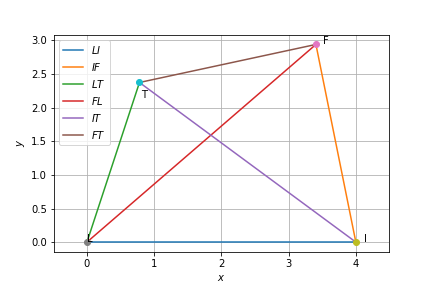
\includegraphics[width= \columnwidth]{quad1.png}
    \caption{Quadrilateral $LIFT$}
\end{figure}
\end{enumerate}
\end{document}